\documentclass{article}
\usepackage{graphicx} % Required for inserting images
\usepackage[russian]{babel}
\usepackage{graphicx}
\usepackage{hyperref}
\title{pr1}
\author{Автор: Ларькин Роман}
\date{16 июля 2025}

\begin{document}
    \title{Мини-конспект по теме: Теорема Пифагора}
\maketitle
\tableofcontents
\newpage
\section{Введение}
\newline{Теорема Пифагора — одна из важнейших теорем евклидовой геометрии. Она находит
 применение в самых разных областях}
\begin{itemize}
    \item геометрия и тригонометрия
    \item физика
    \item инженерные расчёты
    \item компьютерная графика
\end{itemize}

\section{Формулировка теоремы}
\newline{\textbf{Слова}: В прямоугольном треугольнике квадрат гипотенузы равен сумме квадратов
катетов.}
\begin{center}
\newline{$c^2=a^2+b^2$}
\end{center}
\newline{Как видно из формулы 1, знание двух сторон позволяет найти третью.}

\section{Доказательство (набросок)}
\newline {Одно из доказательств основывается на площади квадрата, составленного
из четырёх одинаковых прямоугольных треугольников и малого квадрата
в центре. Раскладывая площадь двумя способами, получаем $c^2=a^2+b^2$.}

\section{Примеры расчёта}
\newline{\textbf{Пример 1}}
\begin{center}
\newline{a = 3, b = 4}
\newline{c = {\sqrt{$a^2+b^2$}} = {\sqrt {9+16} = 5}}
\end{center}
\newline{\textbf{Пример 2}}
\begin{enumerate}
\item Дано: a = 5, b = 12
\item Решение:
\end{enumerate}
\begin{center}
\newline{c = {\sqrt{$a^2+b^2$}} = {\sqrt {25+144} = 13}}
\end{center}

\section{Таблица значений}
\begin{center}
\begin{tabular}{|c|c|c|}
\hline
Катет a & Катет b & Гипотенуза c \\
\hline
3 & 4 & 5 \\
\hline
5 & 12 & 13 \\
\hline
7 & 24 & 25 \\
\hline
\end{tabular}
\end{center}
\section{Иллюстрация}
\newline Ниже пример изображения:
\newline 
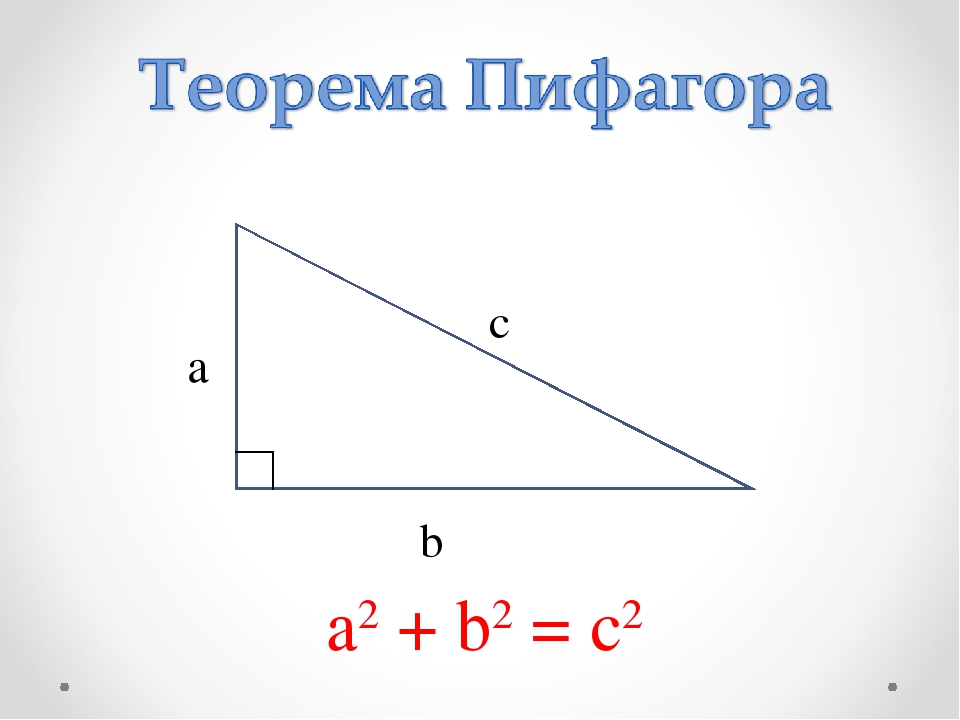
\includegraphics[width=0.5\linewidth]{img5.jpg}
\section{Заключение}
\newline Теорема Пифагора — один из краеугольных камней геометрии, помогающий решать
 множество практических задач.
\section{Ссылки и литература}
\begin{itemize}
    \item Википедия: \href{https://ru.wikipedia.org/wiki/%D0%A2%D0%B5%D0%BE%D1%80%D0%B5%D0%BC%D0%B0_%D0%9F%D0%B8%D1%84%D0%B0%D0%B3%D0%BE%D1%80%D0%B0}{Теорема Пифагора}
    \item Классические учебники геометрии
\end{itemize}
\newpage 
\end{document}